The machine learning experiments conducted in this thesis were performed
using the AI-Hub computational cluster at the University of Oslo. This resource 
consists of three machines with four RTX 2080 Nvidia GPU’s (graphics
processing unit) each. These cards have ~10GB of memory available for the
allocation of models.

\section{Preliminary analysis and comparison of simulated and experimental data}
\begin{figure}
\centering
\includegraphics[width=\textwidth]{chapters/results/figures/comparison_intensity.pdf}
\caption{\label{fig:comparison-intensity}Distributions of total pixel intensities and
highest intensities in experimental and simulated decays. Top row compares experimental 
decays and all simulated decays. The bottom row shows the same distributions, but with simulated
decays split into single and double events. The calculations are done post normalization, so
the maximum possible intensity is 1.0.}
\end{figure}
\begin{figure}
\centering
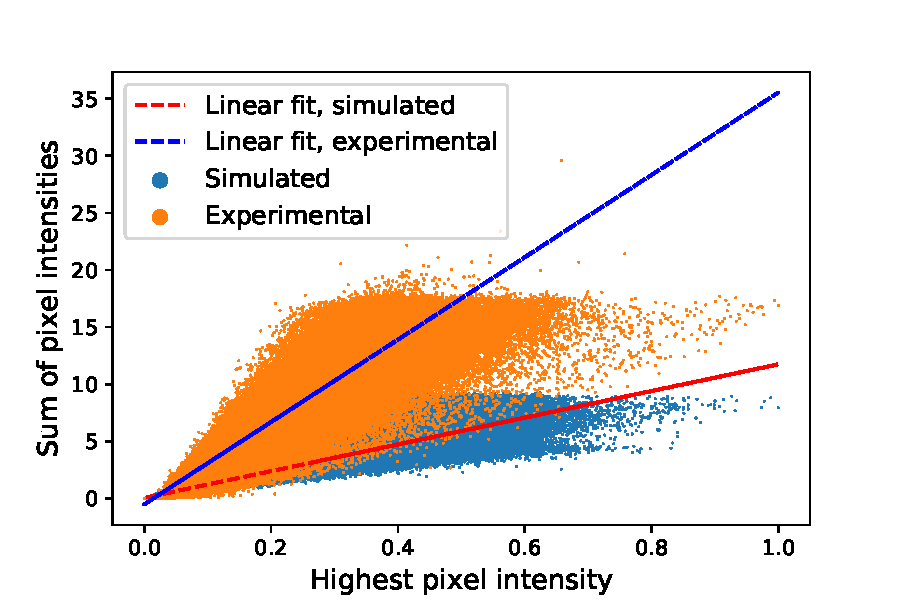
\includegraphics[width=\textwidth]{chapters/results/figures/intensity_hip_comparison.pdf}
\caption{\label{fig:intensity-hip-comparison}Scatterplot of sum of intensities in images vs
the highest intensity in the same image, for both experimental and simulated decays.
Linear fits give slopes of $a_{experimental}=36.05$ and $a_{simulated}=11.69$.}
\end{figure}
\section{Classification}
For classification we have used five different model types,
spanning a range of complexities, architectures, and parameters.
The reason for multiple models is the fundamental difference between the
simulated and experimental datasets; labels. Without ground truth labels
for the experimental data, we need other ways to assess how a model performs in
its task. We attempt to gain some insight by comparing the models' performance on
simulated data with their outputs when applied to experimental data.

\noindent We train the models on three sets of simulated data.
The first (a) is the simulated data as-is, with no changes apart from normalization
and pre-processing. The second (b) is the same data as (a), but with specific pixels in
the 'detector images' set to zero. These pixels are effectively "dead" in the
experimental dataset, and we wish to monitor the effect this has on model performance.
The last dataset (c) has been intentionally imbalanced to further mimick experimental data,
wherein we expect the majority of events to be 'single' events, rather than 'double'
events, as outlined in section \ref{sec:experimental-background}.

\noindent The variability in results is estimated using a K-fold cross-validation approach, with
$K = 5$ \cite{Stone1974}.

\subsection{Classification on simulated data}
As the data consists of detector \textit{images} we expect convolutional
neural networks to be particularly well-suited for the classification task.
In table \ref{tab:classification-simulated-all-f1-auc} the performance of each model
is reported through the estimated $F1$-score, for each of the datasets. 
\begin{table}
\centering
\caption{
Test set F1-scores for classification of simulated datausing multiple models.
Models are trained on a) unmodified data, b) data where specific pixels are set to zero to mimic
'dead' pixels in experimental data, and c) same as b) and imbalanced to mimic experimental data. 
Error estimates are the standard deviation in results from k-fold cross-validation with $K=5$ folds.
}
\label{tab:classification-simulated-all-f1-auc}
\begin{tabular}{llllll}
\toprule
{} &                                            Logistic &                                               Dense &                                       Convolutional &                                    Pretrained VGG16 &                                              Custom \\
\midrule
F1-score (a) &  $\underset{\num{+- 7.727e-03 }  }{\num{ 0.738 } }$ &  $\underset{\num{+- 1.329e-02 }  }{\num{ 0.91 } }$ &  $\underset{\num{+- 6.286e-03 }  }{\num{ 0.964 } }$ &  $\underset{\num{+- 1.591e-02 }  }{\num{ 0.911 } }$ &  $\underset{\num{+- 2.260e-02 }  }{\num{ 0.957 } }$ \\
F1-score (b) &  $\underset{\num{+- 2.273e-03 }  }{\num{ 0.732 } }$ &  $\underset{\num{+- 8.276e-03 }  }{\num{ 0.916 } }$ &  $\underset{\num{+- 3.640e-02 }  }{\num{ 0.758 } }$ &  $\underset{\num{+- 1.926e-02 }  }{\num{ 0.897 } }$ &  $\underset{\num{+- 7.601e-03 }  }{\num{ 0.938 } }$ \\
F1-score (c) &  $\underset{\num{+- 8.483e-02 }  }{\num{ 0.292 } }$ &  $\underset{\num{+- 1.233e-01 }  }{\num{ 0.52 } }$ &  $\underset{\num{+- 9.458e-02 }  }{\num{ 0.9 } }$ &  $\underset{\num{+- 3.606e-02 }  }{\num{ 0.823 } }$ &  $\underset{\num{+- 1.047e-01 }  }{\num{ 0.97 } }$ \\
\bottomrule
\end{tabular}
\end{table}

As a benchmark, we are including a model based on a state of the art pretrained 
network\cite{Simonyan2015}, as outlined in section \ref{sec:method-pretrained}. 
In in figure \ref{fig:confmat-simulated}, we show the confusion matrix for prediction
on test set data for all the models, including normalized values for each event type.
\begin{figure}
\centering
\includegraphics[width=\textwidth]{chapters/results/figures/confmat_simulated.pdf}
\caption{\label{fig:confmat-simulated}Confusion matrices for each model trained
on simulated data. For each model and dataset, the number of events and ratio of each
event type are given. a) unmodified data. b) select pixels set to zero. c) Same as in b)
with the intentionally imbalanced.}
\end{figure}. The F1-scores show decreasing
performance for most models when applying modifications to the original simulated dataset.
For the CNN the effect is more severe. When training on an intentionally imbalanced
dataset the models without CNN architechtures show a significant decrease in performance.
Considering the confusion matrix we see that the logistic regressor and dense network
suffer from predicting mostly every sample to be single events. Looking back to the
$F1$-scores again, there is not a significant increase in performance between the
CNN and the Custom model on unmodified data, but the custom model performs strongly
across all datasets, with a lowY amount of misclassified events relative to the other
models.

\subsection{Classification on experimental data}
Classification of experimental data poses a different set of challenges when it comes
to evaluating our results. We only have a handful of events that are handlabeled as
double events, which can be used as a form of verification. As mentioned in section
\ref{sec:experimental-background}, we expect the number of double events in the experimental
data to be much lower than single events. Inspecting the ratio of predicted singles to predicted
doubles can then be an initial indication of how a model is performing. It is, however,
not conclusive. Correctly classified handlabeled events are another indication, but
is also not conclusive. In table \ref{tab:classification-experimental-ratios}, the ratios
of predicted singles to predicted doubles are presented for each model trained on each
dataset. The actual number of predictions for each class are included below the ratios.

\begin{table}
\centering
\caption{
Decay event classification on experimental data, with models trained on:
a) unmodified data, b) data where specific pixels are set to zero to mimic
'dead' pixels in experimental data, and c) same as b) and imbalanced to mimic experimental data.
}
\label{tab:classification-experimental-ratios}
\begin{tabular}{llll}
\toprule
{} &                                                                    Ratio single, double (a) &         Ratio single, double (b) &          Ratio single, double (c) \\
\midrule
Logistic   &  $\underset{\num{ 198210 }  }{\num{ 0.762 } }, \underset{\num{ 61937 }  }{\num{ 0.238 } }$ &  $\num{ 0.778 }, \num{ 0.222 }$ &  $\num{ 1 }, \num{ 7.69e-06 }$ \\
Dense      &  $\underset{\num{ 97487 }  }{\num{ 0.375 } }, \underset{\num{ 162660 }  }{\num{ 0.625 } }$ &  $\num{ 0.387 }, \num{ 0.613 }$ &  $\num{ 1 }, \num{ 9.61e-05 }$ \\
CNN        &  $\underset{\num{ 63051 }  }{\num{ 0.242 } }, \underset{\num{ 197096 }  }{\num{ 0.758 } }$ &  $\num{ 0.257 }, \num{ 0.743 }$ &  $\num{ 0.379 }, \num{ 0.621 }$ \\
Pretrained &  $\underset{\num{ 138614 }  }{\num{ 0.533 } }, \underset{\num{ 121533 }  }{\num{ 0.467 } }$ &  $\num{ 0.53 }, \num{ 0.47 }$ &  $\num{ 0.997 }, \num{ 0.00269 }$ \\
Custom     &  $\underset{\num{ 26277 }  }{\num{ 0.101 } }, \underset{\num{ 233870 }  }{\num{ 0.899 } }$ &  $\num{ 0.0951 }, \num{ 0.905 }$ &  $\num{ 0.204 }, \num{ 0.796 }$ \\
\bottomrule
\end{tabular}
\end{table}

\begin{table}
\centering
\caption{
Decay event classification on 17 labeled samples of experimental data. The 17 samples are all
labeled as double events. Models are trained on simulated data with a varying degree of modification:
a) unmodified data, b) data where specific pixels are set to zero to mimic
'dead' pixels in experimental data, and c) same as b) and imbalanced to mimic experimental data.
The numbers are shown as the normalized ratio of predicted event type, with the actual amount of
events predicted of that type below.
}
\label{tab:classification-experimental-labeled-doubles}
\begin{tabular}{lllllll}
\toprule
{} &                                Single (a) &                                 Double (a) &                                Single (b) &                                 Double (b) &                                Single (c) &                                 Double (c) \\
\midrule
Logistic   &  $\underset{\num{ 0 }  }{\num{ 0.000 } }$ &  $\underset{\num{ 17 }  }{\num{ 1.000 } }$ &  $\underset{\num{ 0 }  }{\num{ 0.000 } }$ &  $\underset{\num{ 17 }  }{\num{ 1.000 } }$ &  $\underset{\num{ 1 }  }{\num{ 0.059 } }$ &  $\underset{\num{ 16 }  }{\num{ 0.941 } }$ \\
Dense      &  $\underset{\num{ 0 }  }{\num{ 0.000 } }$ &  $\underset{\num{ 17 }  }{\num{ 1.000 } }$ &  $\underset{\num{ 0 }  }{\num{ 0.000 } }$ &  $\underset{\num{ 17 }  }{\num{ 1.000 } }$ &  $\underset{\num{ 0 }  }{\num{ 0.000 } }$ &  $\underset{\num{ 17 }  }{\num{ 1.000 } }$ \\
CNN        &  $\underset{\num{ 0 }  }{\num{ 0.000 } }$ &  $\underset{\num{ 17 }  }{\num{ 1.000 } }$ &  $\underset{\num{ 0 }  }{\num{ 0.000 } }$ &  $\underset{\num{ 17 }  }{\num{ 1.000 } }$ &  $\underset{\num{ 0 }  }{\num{ 0.000 } }$ &  $\underset{\num{ 17 }  }{\num{ 1.000 } }$ \\
Pretrained &  $\underset{\num{ 0 }  }{\num{ 0.000 } }$ &  $\underset{\num{ 17 }  }{\num{ 1.000 } }$ &  $\underset{\num{ 0 }  }{\num{ 0.000 } }$ &  $\underset{\num{ 17 }  }{\num{ 1.000 } }$ &  $\underset{\num{ 3 }  }{\num{ 0.176 } }$ &  $\underset{\num{ 14 }  }{\num{ 0.824 } }$ \\
Custom     &  $\underset{\num{ 0 }  }{\num{ 0.000 } }$ &  $\underset{\num{ 17 }  }{\num{ 1.000 } }$ &  $\underset{\num{ 0 }  }{\num{ 0.000 } }$ &  $\underset{\num{ 17 }  }{\num{ 1.000 } }$ &  $\underset{\num{ 0 }  }{\num{ 0.000 } }$ &  $\underset{\num{ 17 }  }{\num{ 1.000 } }$ \\
\bottomrule
\end{tabular}
\end{table}

\begin{figure}
\centering
\includegraphics[width=\textwidth]{chapters/results/figures/classification_experimental_single_fractions.pdf}
\caption{\label{fig:experimental-single-fractions}Fraction of predicted singles as a function of
total intensity in images, for each model trained on simulated data.  a) unmodified data. b) select pixels set to zero. 
c) Same as in b) with the intentionally imbalanced.}
\end{figure}
\begin{figure}
\centering
\includegraphics[width=\textwidth]{chapters/results/figures/simulated_scaled_intensity.pdf}
\caption{\label{fig:simulated-scaled-intensities}Fraction of simulated single events correctly classified
as a function of scaling factor used to increase the total intensity in simulated decays. In the title of
each plot is the dataset the models were trained on. The dataset used for prediction is dataset $a$.}
\end{figure}
 
\section{Regression}
\subsection{Regression on simulated data}
On data already classified, we attempt to predict the energy of the events and the 
position of origin for the electrons. Because there is a travel distance between the 
ejection site and the point the energy is deposited, the positions aren't necessarily
the locations of the highest-intensity pixels in the detector images.
Note that for regression the models are trained on single or double events exclusively.
This means that for dataset $(c)$, which is imbalanced, the set of single events is
identical to that of set $(b)$, causing near-identical results between these two sets.
Due to the poor performance of models trained on simulated double events, and the
expected low frequency of double events in the experimental data, we only apply models
trained on simulated single events.
\subsubsection{Position of origin}
In table \ref{tab:regression-simulated-all-positions-r2} the R2-scores for all models
trained on simulated data are presented. A similar trend as was seen for classification
can be observed for single events, where models are trained on unmodified data. Even
a linear regressor is able to predict positions of origin fairly well, but it is clear
that the neural networks perform at a much higher level in this case. They have strong
R2-scores of 0.99 and higher, and very little degradation in performance with added 
modifications to the training data. Again, as with classification, the custom model
performs strongly across all datasets for single events.
In the case of regression on double events, none of the models are able to accurately
predict positions of origins for both events.
\begin{table}
\centering
\caption{
Test set R2-scores for regresson of positions of origin on simulated data, with models trained on data with: 
a) no modifications, b) specific pixels set to zero to mimic experimental data, and c) imbalanced dataset
in addition to modifications in b) to further mimic experimental data. Error estimates are the standard deviation 
in results from validation data in k-fold cross-validation with $K=5$ folds.
}
\label{tab:regression-simulated-all-positions-r2}
\begin{tabular}{llllll}
\toprule
{} &                                              Linear &                                               Dense &                                                 CNN &                                          Pretrained &                                                  Custom \\
\midrule
Single (a) &  $\underset{\num{+- 2.871e-03 }  }{\num{ 0.8 } }$ &  $\underset{\num{+- 1.101e-03 }  }{\num{ 0.986 } }$ &  $\underset{\num{+- 5.085e-03 }  }{\num{ 0.997 } }$ &  $\underset{\num{+- 6.945e-02 }  }{\num{ 0.826 } }$ &  $\underset{\num{+- 4.469e-01 }  }{\num{ -6.15e-05 } }$ \\
Single (b) &  $\underset{\num{+- 2.737e-03 }  }{\num{ 0.776 } }$ &  $\underset{\num{+- 6.798e-04 }  }{\num{ 0.987 } }$ &  $\underset{\num{+- 1.015e-03 }  }{\num{ 0.988 } }$ &  $\underset{\num{+- 1.723e-02 }  }{\num{ 0.873 } }$ &  $\underset{\num{+- 2.114e-04 }  }{\num{ 0.997 } }$ \\
Single (c) &  $\underset{\num{+- 2.725e-03 }  }{\num{ 0.776 } }$ &  $\underset{\num{+- 1.550e-03 }  }{\num{ 0.98 } }$ &  $\underset{\num{+- 5.303e-03 }  }{\num{ 0.94 } }$ &  $\underset{\num{+- 2.695e-01 }  }{\num{ 0.475 } }$ &  $\underset{\num{+- 4.464e-01 }  }{\num{ -7.12e-05 } }$ \\
Double (a) &  $\underset{\num{+- 5.796e-03 }  }{\num{ 0.364 } }$ &  $\underset{\num{+- 1.389e-02 }  }{\num{ 0.435 } }$ &  $\underset{\num{+- 1.945e-03 }  }{\num{ 0.47 } }$ &  $\underset{\num{+- 2.085e-03 }  }{\num{ 0.24 } }$ &  $\underset{\num{+- 2.711e-01 }  }{\num{ -0.000341 } }$ \\
Double (b) &  $\underset{\num{+- 6.804e-04 }  }{\num{ 0.365 } }$ &  $\underset{\num{+- 8.661e-04 }  }{\num{ 0.466 } }$ &  $\underset{\num{+- 1.841e-03 }  }{\num{ 0.363 } }$ &  $\underset{\num{+- 1.397e-02 }  }{\num{ 0.343 } }$ &  $\underset{\num{+- 2.694e-04 }  }{\num{ 0.488 } }$ \\
Double (c) &  $\underset{\num{+- 7.794e-03 }  }{\num{ 0.357 } }$ &  $\underset{\num{+- 7.345e-03 }  }{\num{ 0.422 } }$ &  $\underset{\num{+- 4.092e-03 }  }{\num{ 0.449 } }$ &  $\underset{\num{+- 1.031e-02 }  }{\num{ 0.437 } }$ &  $\underset{\num{+- 2.648e-01 }  }{\num{ -0.00801 } }$ \\
\bottomrule
\end{tabular}
\end{table}

\subsubsection{Energy}
In table \ref{tab:regression-simulated-all-energies-r2} the R2-scores for all models
trained on simulated data are presented.
Performance when predicting single energies is across the board lower when compared with
R2-scores for positions. On unmodified data the models are to a large degree able to
predict energies, with R2-score of 0.93 and above. For the modified datasets the CNN
suffers greatly and isn't able to predict energies at all. Other models see a less
severe effect, but still a clear reduction in performance.
As was the case with prediction of positions, no models predict energies
of double events with any useful degree of accuracy.
\begin{table}
\centering
\caption{
Test set R2-scores for regresson of energies on simulated data, with models trained on data with: 
a) no modifications, b) specific pixels set to zero to mimic experimental data, and c) imbalanced dataset
in addition to modifications in b) to further mimic experimental data. Error estimates are the standard deviation 
in results from validation data in k-fold cross-validation with $K=5$ folds.
}
\label{tab:regression-simulated-all-energies-r2}
\begin{tabular}{llllll}
\toprule
{} &                                              Linear &                                               Dense &                                                  CNN &                                          Pretrained &                                                  Custom \\
\midrule
Single (a) &  $\underset{\num{+- 3.691e-02 }  }{\num{ 0.936 } }$ &  $\underset{\num{+- 3.578e-02 }  }{\num{ 0.936 } }$ &  $\underset{\num{+- 3.440e-02 }  }{\num{ 0.942 } }$ &  $\underset{\num{+- 3.734e-02 }  }{\num{ 0.932 } }$ &  $\underset{\num{+- 4.101e-01 }  }{\num{ -3.16e-06 } }$ \\
Single (b) &  $\underset{\num{+- 2.459e-02 }  }{\num{ 0.739 } }$ &  $\underset{\num{+- 2.261e-02 }  }{\num{ 0.754 } }$ &  $\underset{\num{+- 2.405e-02 }  }{\num{ -0.128 } }$ &  $\underset{\num{+- 1.418e-02 }  }{\num{ 0.728 } }$ &  $\underset{\num{+- 2.865e-02 }  }{\num{ 0.733 } }$ \\
Single (c) &  $\underset{\num{+- 2.459e-02 }  }{\num{ 0.739 } }$ &  $\underset{\num{+- 2.422e-02 }  }{\num{ 0.753 } }$ &  $\underset{\num{+- 2.710e-02 }  }{\num{ 0.581 } }$ &  $\underset{\num{+- 1.999e-02 }  }{\num{ 0.77 } }$ &  $\underset{\num{+- 4.327e-01 }  }{\num{ 0.778 } }$ \\
Double (a) &  $\underset{\num{+- 3.347e-02 }  }{\num{ 0.49 } }$ &  $\underset{\num{+- 3.087e-02 }  }{\num{ 0.49 } }$ &  $\underset{\num{+- 4.257e-02 }  }{\num{ 0.488 } }$ &  $\underset{\num{+- 2.398e-02 }  }{\num{ 0.491 } }$ &  $\underset{\num{+- 2.091e-01 }  }{\num{ -0.000157 } }$ \\
Double (b) &  $\underset{\num{+- 3.155e-03 }  }{\num{ 0.487 } }$ &  $\underset{\num{+- 2.571e-03 }  }{\num{ 0.49 } }$ &  $\underset{\num{+- 3.120e-03 }  }{\num{ 0.282 } }$ &  $\underset{\num{+- 1.032e-02 }  }{\num{ 0.455 } }$ &  $\underset{\num{+- 2.746e-03 }  }{\num{ 0.466 } }$ \\
Double (c) &  $\underset{\num{+- 4.613e-02 }  }{\num{ 0.411 } }$ &  $\underset{\num{+- 4.563e-02 }  }{\num{ 0.432 } }$ &  $\underset{\num{+- 5.390e-02 }  }{\num{ 0.461 } }$ &  $\underset{\num{+- 2.682e-02 }  }{\num{ 0.44 } }$ &  $\underset{\num{+- 2.091e-01 }  }{\num{ 0.412 } }$ \\
\bottomrule
\end{tabular}
\end{table}


\subsection{Regression on experimental data}
\begin{figure}
\centering
\includegraphics[width=\textwidth]{chapters/results/figures/experimental_pos_dist.pdf}
\caption{\label{fig:experimental-pos-dist} Distribution of distances between predicted
positions of origin and the highest intensity pixel(HIP) in the corresponding images. 
The model was a custom cnn architecture, trained on simulated data where (b) denotes 
that elect pixels were set to zero across the dataset. This model was selected for this
plot due to it having the lowest mean distance from HIP.}
\end{figure}
\begin{table}
\centering
\caption{
Mean distances of predicted position of origin on experimental decays, to center of highest intensity pixel (HIP).Models 
trained on data with: a) no modifications, b) specific pixels set to zero to mimic experimental data, and c) imbalanced dataset
in addition to modifications in b) to further mimic experimental data.
}
\label{tab:regression-experimental-dist-means}
\begin{tabular}{ll}
\toprule
{} & Mean distance [mm] \\
\midrule
LinReg (a)     &  $\num{ 17.61 }$ \\
Dense (a)      &  $\num{ 16.89 }$ \\
CNN (a)        &  $\num{ 12.53 }$ \\
Pretrained (a) &  $\num{ 4.59 }$ \\
Custom (a)     &  $\num{ 3.88 }$ \\
LinReg (b)     &  $\num{ 17.49 }$ \\
Dense (b)      &  $\num{ 13.80 }$ \\
CNN (b)        &  $\num{ 12.49 }$ \\
Pretrained (b) &  $\num{ 4.80 }$ \\
Custom (b)     &  $\num{ 3.50 }$ \\
LinReg (c)     &  $\num{ 17.49 }$ \\
Dense (c)      &  $\num{ 13.79 }$ \\
CNN (c)        &  $\num{ 12.40 }$ \\
Pretrained (c) &  $\num{ 4.66 }$ \\
Custom (c)     &  $\num{ 3.48 }$ \\
\bottomrule
\end{tabular}
\end{table}
